\documentclass{article}
\usepackage{tikz}
\usetikzlibrary{shapes, arrows.meta, positioning}
\tikzstyle{process} = [rectangle, 
minimum width=3cm, 
minimum height=1cm, 
text centered, 
text width=3cm, 
draw=black, 
fill=orange!30]

\tikzstyle{decision} = [diamond, 
minimum width=3cm, 
minimum height=1cm, 
text centered, 
draw=black, 
fill=green!30]
\tikzset{
    %process/.style = {rectangle, draw, text width=6em, text centered, minimum height=1.5em},
    %decision/.style = {diamond, draw, text width=5.5em, text centered, aspect=2, minimum height=1.5em},
    answer/.style = {rectangle, draw, text width=2em, text centered, minimum height=1em, fill=gray!20},
    arrow/.style = {thick, -Stealth}
}

\begin{document}
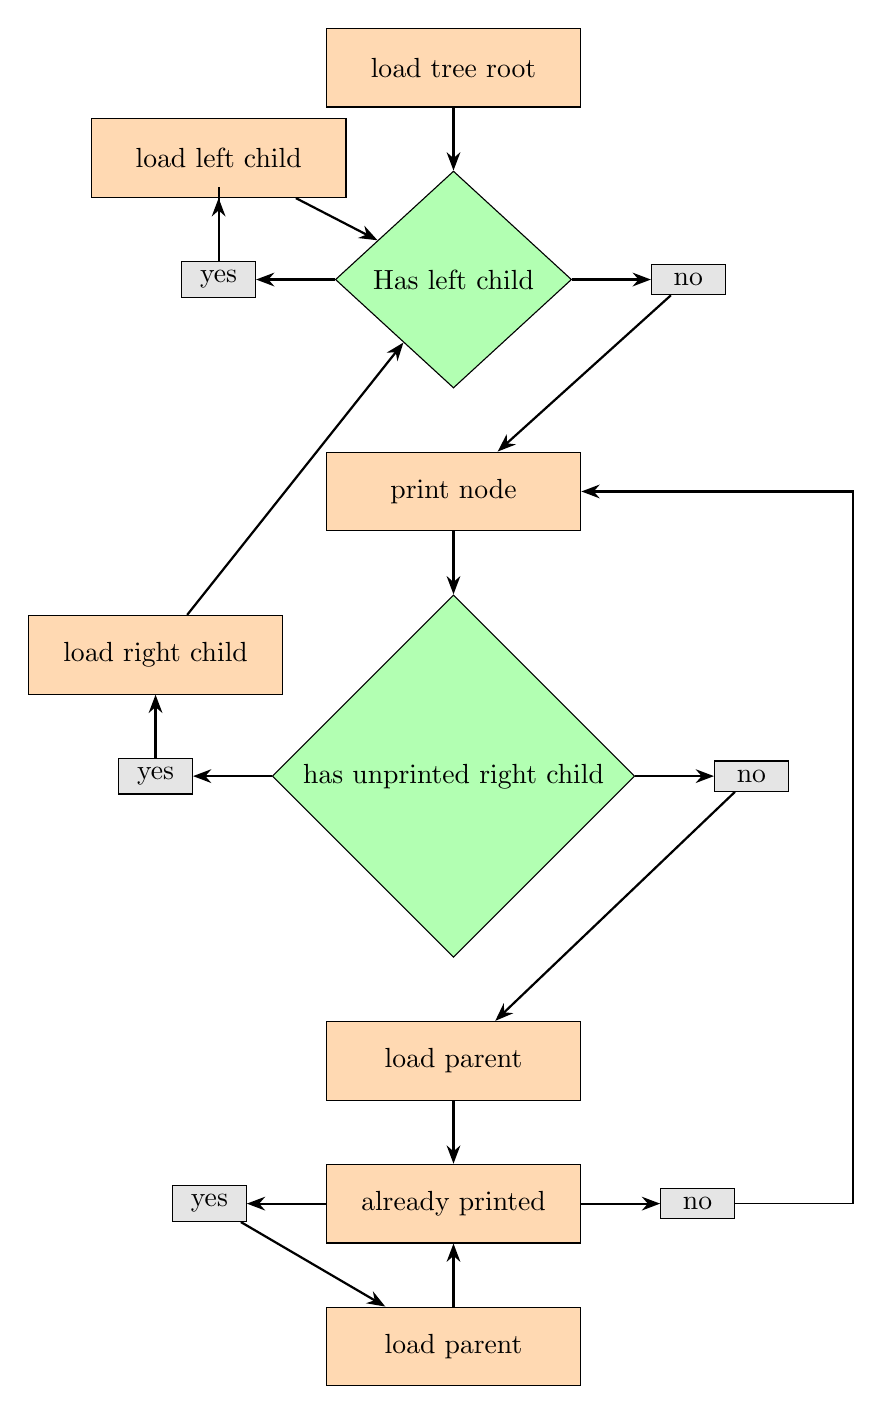
\begin{tikzpicture}[node distance=0.8cm and 1cm]

% Nodes
\node (load1) [process] {load tree root};
\node (decision1) [decision, below=of load1] {Has left child};
\node (yes1) [answer, left=of decision1] {yes};
\node (no1) [answer, right=of decision1] {no};
\node (print1) [process, above=of yes1] {load left child};
\node (print) [process, below=of decision1] {print node};
\node (decision2) [decision, below=of print] {has unprinted right child};
\node (no2) [answer, left=of decision2] {yes};
\node (yes2) [answer, right=of decision2] {no};
\node (load2) [process, below=of decision2] {load parent};
\node (print2) [process, below=of load2] {already printed};
\node (yes3) [answer, left=of print2] {yes};
\node (no3) [answer, right=of print2] {no};
\node (load3) [process, below=of print2] {load parent};
\node (load4) [process, above=of no2] {load right child};


% Arrows
\draw [arrow] (print1) -- (decision1);
\draw [arrow] (load1) -- (decision1);
\draw [arrow] (decision1) -- (yes1);
\draw [arrow] (decision1) -- (no1);
\draw [arrow] (yes1) |- (print1.south);
\draw [arrow] (no1) -- (print);
\draw [arrow] (print) -- (decision2);
\draw [arrow] (decision2) -- (yes2);
\draw [arrow] (decision2) -- (no2);
\draw [arrow] (yes2) -- (load2);
\draw [arrow] (no2) -- (load4.south);
\draw [arrow] (load4) -- (decision1);
\draw [arrow] (load2) -- (print2);
\draw [arrow] (print2) -- (yes3);
\draw [arrow] (print2) -- (no3);
\draw [arrow] (yes3) -- (load3);
\draw [arrow] ([xshift=1.5cm]no3.east) |- (print.east);
\draw [arrow] (load3) -- (print2);
\draw []  (no3.east) -- ([xshift=1.5cm]no3.east);

\end{tikzpicture}
\end{document}